% ============================================================
% EC8208 - Software Architecture
% Continuous Assessment 01 - Architecture Analysis and Design Report
% Domain: Clinic Appointment Booking (offline visit)  |  Style: Microservices
% Compile with: pdflatex (run twice for ToC/cross-references)
% ============================================================
\documentclass[12pt,a4paper]{article}

% ---------- Fonts: Times New Roman look-alike ----------
\usepackage{newtxtext,newtxmath}
\usepackage[T1]{fontenc}
\usepackage[utf8]{inputenc}

% ---------- Geometry & spacing ----------
\usepackage[a4paper,margin=1in]{geometry}
\usepackage{setspace}
\onehalfspacing % 1.5 line spacing

% ---------- Packages ----------
\usepackage{graphicx}
\usepackage{xcolor}
\usepackage{array}
\usepackage{longtable}
\usepackage{booktabs}
\usepackage{tabularx}
\usepackage{enumitem}
\usepackage{titlesec}
\usepackage{fancyhdr}
\usepackage{caption}
\usepackage{float}
\usepackage[hidelinks]{hyperref}

% ---------- TikZ for diagrams ----------
\usepackage{tikz}
\usetikzlibrary{shapes.geometric,shapes.multipart,arrows.meta,positioning,fit,backgrounds,calc,shadows}

% ---------- Colors ----------
\definecolor{navy}{RGB}{20,52,95}
\definecolor{steel}{RGB}{52,101,164}
\definecolor{lightblue}{RGB}{222,235,247}
\definecolor{softgreen}{RGB}{226,240,217}
\definecolor{softorange}{RGB}{252,235,219}
\definecolor{softgray}{RGB}{237,237,237}
\definecolor{softpurple}{RGB}{233,226,245}

% ---------- Section formatting ----------
\titleformat{\section}{\normalfont\Large\bfseries\color{navy}}{\thesection.}{0.6em}{}
\titleformat{\subsection}{\normalfont\large\bfseries\color{steel}}{\thesubsection}{0.6em}{}
\titleformat{\subsubsection}{\normalfont\normalsize\bfseries}{\thesubsubsection}{0.6em}{}

% ---------- Table caption style ----------
\captionsetup{font=small,labelfont=bf}

% ---------- Header/Footer ----------
\setlength{\headheight}{14pt}
\pagestyle{fancy}
\fancyhf{}
\renewcommand{\headrulewidth}{0.4pt}
\fancyhead[L]{\small EC8208 : Software Architecture}
\fancyhead[R]{\small CA01: Architecture Report}
\fancyfoot[C]{\small\thepage}

\setlength{\parskip}{0.5em}
\setlength{\parindent}{0pt}

% ---------- TikZ reusable styles ----------
\tikzset{
  box/.style={rectangle,rounded corners=2pt,draw=navy,thick,fill=lightblue,
              minimum width=2.6cm,minimum height=0.9cm,align=center,font=\small},
  svc/.style={rectangle,rounded corners=2pt,draw=steel,thick,fill=softgreen,
              minimum width=2.4cm,minimum height=0.9cm,align=center,font=\small},
  store/.style={cylinder,shape border rotate=90,aspect=0.25,draw=navy,thick,
              fill=softorange,minimum width=2cm,minimum height=1.1cm,align=center,font=\footnotesize},
  ext/.style={rectangle,draw=gray,thick,fill=softgray,minimum width=2.4cm,
              minimum height=0.9cm,align=center,font=\small},
  actor/.style={align=center,font=\small},
  flow/.style={-{Stealth[length=2.5mm]},thick,draw=navy},
  flowg/.style={-{Stealth[length=2.5mm]},thick,draw=steel,dashed},
}

% ============================================================
\begin{document}

% ---------------- TITLE PAGE ----------------
\begin{titlepage}
\centering
\vspace*{0.6cm}
{\Large Department of Computer Engineering\par}
\vspace{0.3cm}
{\large EC8208 : Software Architecture\par}
\vspace{1.4cm}

\rule{\linewidth}{0.5mm}\par
\vspace{0.5cm}
{\Huge\bfseries\color{navy} Architecture Analysis and Design Report\par}
\vspace{0.4cm}
{\LARGE A Microservices-Based Clinic Appointment Booking Platform\par}
\vspace{0.3cm}
{\large ``MediConnect'' : Clinic Appointment Booking System\par}
\vspace{0.5cm}
\rule{\linewidth}{0.5mm}\par

\vspace{1.0cm}
{\large Continuous Assessment 01\par}
\vspace{0.2cm}
{\large Group Take-Home Assessment\par}

\vfill

{\large\bfseries Group Members\par}
\vspace{0.4cm}
{\renewcommand{\arraystretch}{1.35}
\begin{tabular}{ll}
EG/2021/4487 & Dinojan V.\\
EG/2021/4566 & Jackshan Venujan G.S.\\
EG/2021/4825 & Tharshihan R.\\
EG/2021/4590 & Jegan T.\\
EG/2021/4434 & Bandara M.M.D.L.\\
\end{tabular}\par}

\vspace{0.9cm}
{\large Date of Submission: July 13, 2026\par}
\vspace{0.4cm}
\end{titlepage}

% ---------------- TABLE OF CONTENTS ----------------
\tableofcontents
\thispagestyle{fancy}
\newpage

% ============================================================
\section{Introduction}

\subsection{Background of the Selected Problem}
In many clinics and hospitals, patients still book appointments by phone or by walking in and
waiting in long queues. There is often no easy way to see which doctor is available, at which
clinic, and at what time. This leads to long waiting times, overbooking, missed appointments,
and poor use of doctors' time. Most patients would prefer to arrange a visit in advance and
then attend the clinic at a fixed time, instead of waiting for hours.

A web-based appointment booking platform can address this. Through a web application, a patient
can find a suitable doctor and clinic, view the available time slots, and book an appointment in
advance. The patient then visits the clinic in person at the booked time for the consultation.
The clinic and its doctors manage their schedules, record each visit, and issue prescriptions
through the same system. This keeps the booking process organised and reduces waiting, while the
consultation itself remains face to face at the clinic.

\subsection{Problem Statement}
Manual, phone-based, or walk-in appointment handling at clinics causes long queues,
double-booking, and no clear view of doctor availability. Paper-based records also make it hard
to track a patient's history across visits. \textbf{There is a clear need for a secure,
scalable, and highly available web platform that lets patients book appointments with clinic
doctors in advance and attend in person, while giving doctors and administrators the tools to
manage schedules, records, and prescriptions reliably as the number of clinics, doctors, and
patients grows.}

\subsection{Objectives of the Proposed System}
The proposed system, \textbf{MediConnect}, focuses on a core, achievable set of objectives:
\begin{itemize}[leftmargin=1.4em,itemsep=2pt]
  \item Allow patients, doctors, and administrators to register and log in with role-based
        access.
  \item Let patients search for doctors and clinics by speciality and location, and view the
        available time slots.
  \item Let patients book, reschedule, or cancel an appointment at a physical clinic for a
        chosen time slot.
  \item After the in-clinic visit, let doctors record consultation notes and issue digital
        prescriptions that patients can view and download.
  \item Send appointment confirmations and reminders, and handle the booking or consultation
        fee through a secure payment step.
  \item Keep patient data confidential and available, and keep the system modular so that it
        can scale as more clinics and doctors join.
\end{itemize}

% ============================================================
\section{Requirements Analysis}

\subsection{Functional Requirements}
\begin{longtable}{>{\bfseries}p{1.6cm} p{3.2cm} p{8.2cm}}
\caption{Functional requirements of MediConnect.}\\
\toprule
\textbf{ID} & \textbf{Requirement} & \textbf{Description}\\
\midrule
\endfirsthead
\toprule
\textbf{ID} & \textbf{Requirement} & \textbf{Description}\\
\midrule
\endhead
FR-01 & User Registration \& Authentication & Patients, doctors, and administrators can
register, verify their identity, and log in using credentials secured by token-based
authentication.\\
FR-02 & Doctor \& Clinic Search & Patients can search and filter doctors by speciality, clinic,
and location, and view each doctor's availability.\\
FR-03 & Appointment Booking & Patients can view a doctor's available time slots at a clinic and
book, reschedule, or cancel a physical appointment.\\
FR-04 & Consultation Record & After the in-clinic visit, the doctor records the consultation
notes and the visit outcome in the system.\\
FR-05 & E-Prescription & Doctors can create and digitally sign prescriptions that patients can
view and download.\\
FR-06 & Electronic Health Records & The system stores and retrieves each patient's visit
history, prescriptions, and consultation notes.\\
FR-07 & Payment Processing & Patients pay the booking or consultation fee through a secure
payment step and receive a receipt.\\
FR-08 & Notifications & The system sends appointment confirmations and reminders via email and
SMS.\\
FR-09 & Rating \& Feedback & Patients can rate and review doctors after a completed visit.\\
FR-10 & Administration & Administrators can verify doctor credentials, manage clinics and
users, and monitor platform activity.\\
\bottomrule
\end{longtable}

\subsection{Non-Functional Requirements}
The following non-functional requirements define the quality attributes the system must meet.
They are the main drivers of the architectural decisions in this report.
\begin{longtable}{>{\bfseries}p{1.6cm} p{3.2cm} p{8.2cm}}
\caption{Non-functional requirements of MediConnect.}\\
\toprule
\textbf{ID} & \textbf{Attribute} & \textbf{Requirement}\\
\midrule
\endfirsthead
\toprule
\textbf{ID} & \textbf{Attribute} & \textbf{Requirement}\\
\midrule
\endhead
NFR-01 & Scalability & The platform shall scale horizontally to support at least 10{,}000
concurrent users during peak booking hours.\\
NFR-02 & Performance & 95\% of API requests shall respond within 500\,ms under nominal load.\\
NFR-03 & Security & All data in transit shall use TLS 1.2+; sensitive data at rest shall be
encrypted; access shall be role-based.\\
NFR-04 & Availability & The system shall maintain 99.9\% uptime, with no single point of
failure for core services.\\
NFR-05 & Reliability & Appointment, payment, and prescription operations shall be
transactionally consistent and recoverable after failure.\\
NFR-06 & Maintainability & Services shall be independently deployable, with clear interfaces,
to allow isolated updates.\\
NFR-07 & Privacy/Compliance & The platform shall comply with health-data protection
principles (for example, HIPAA or GDPR style consent and audit logging).\\
NFR-08 & Usability & The user interface shall be responsive and accessible on modern web
browsers.\\
NFR-09 & Interoperability & The system shall expose RESTful APIs and support integration
with external pharmacy and laboratory systems.\\
\bottomrule
\end{longtable}

\subsection{Stakeholder Identification}
The table below identifies the parties whose needs drive the requirements above.
\begin{longtable}{>{\bfseries}p{3.2cm} p{10.8cm}}
\caption{Key stakeholders and their roles.}\\
\toprule
\textbf{Stakeholder} & \textbf{Interest / Role}\\
\midrule
\endfirsthead
\toprule
\textbf{Stakeholder} & \textbf{Interest / Role}\\
\midrule
\endhead
Patients & Primary end users who book appointments in advance and attend the clinic in person.\\
Doctors & Manage their schedules, see booked appointments, and record visit notes and
prescriptions.\\
Clinics & Provide the physical location and doctors, and manage their listed availability.\\
Administrators & Verify doctors, manage clinics and users, and monitor platform health and
compliance.\\
Pharmacies \& Labs & External partners fulfilling prescriptions and diagnostic orders.\\
Payment Provider & Third-party service that processes booking and consultation payments.\\
Regulators & Authorities enforcing health-data privacy and clinical compliance.\\
Development \& Ops Team & Build, deploy, scale, and maintain the platform.\\
\bottomrule
\end{longtable}

% ============================================================
\section{Architecture Selection}

\subsection{Candidate Architecture Styles}
Several common architecture styles were evaluated against the requirements above. Because each
style involves trade-offs, the options are judged by how well they serve this system's goals
rather than by any single style being best in general.

\begin{longtable}{p{2.7cm} p{5.0cm} p{5.4cm}}
\caption{Comparison of candidate architecture styles.}\\
\toprule
\textbf{Style} & \textbf{Strengths} & \textbf{Weaknesses for this domain}\\
\midrule
\endfirsthead
\toprule
\textbf{Style} & \textbf{Strengths} & \textbf{Weaknesses for this domain}\\
\midrule
\endhead
Monolithic / Layered (N-tier) & Simple to build and deploy; clear separation of
presentation, business, and data layers; low initial complexity. & A single deployable unit
scales as a whole, couples unrelated concerns, and one failure can bring down the entire
system, which is a poor fit for 99.9\% availability and independent scaling.\\
Client-Server & Well-understood request and response model; centralises data and logic. &
On its own it does not address independent scaling or fault isolation of distinct functions
such as booking and payment.\\
Event-Driven & Excellent for asynchronous, loosely coupled flows such as notifications and
audit logging. & Harder to reason about end-to-end consistency, and it does not by itself
structure the synchronous request and response core (booking, payment).\\
\textbf{Microservices} & Small, independent services that are separately scalable and
deployable, with fault isolation, per-service technology choice, and clear team ownership. &
Higher operational complexity (orchestration, distributed data, networking).\\
\bottomrule
\end{longtable}

\subsection{Selected Style and Justification}
\textbf{MediConnect adopts a Microservices architecture}, supported by an event-driven message
bus for asynchronous tasks, an API Gateway as the single client-facing entry point, and a
layered organisation inside each service. This is a key architectural decision that shapes the
technology, component structure, and integration of the whole system. The justification
follows from the requirements and goals:

\begin{itemize}[leftmargin=1.4em,itemsep=2pt]
  \item \textbf{Independent scalability (NFR-01).} The appointment booking service can be
        scaled on its own during peak booking times, separately from lighter services such as
        prescriptions.
  \item \textbf{Fault isolation and availability (NFR-04).} A failure in the payment service
        must not stop patients from booking or doctors from recording a visit; service
        boundaries contain failures.
  \item \textbf{Maintainability (NFR-06).} Each service has a single responsibility and
        communicates only through published interfaces, which allows isolated, frequent
        deployments.
  \item \textbf{Security (NFR-03).} A central API Gateway enforces authentication, rate
        limiting, and TLS termination uniformly, while sensitive services sit behind it.
  \item \textbf{Asynchronous decoupling.} A message broker carries events (for example,
        \texttt{AppointmentBooked}) to the notification and records services without blocking
        the main request path.
\end{itemize}

Each service owns its own database (the database-per-service pattern), which prevents hidden
coupling through a shared schema and lets each store be tuned for its workload.

% ============================================================
\section{Architectural Design}
The proposed architecture is presented below through a set of standard design diagrams.

\subsection{Context Diagram}
The context diagram shows MediConnect as a single system and its interactions with external
actors and systems.

\begin{figure}[H]
\centering
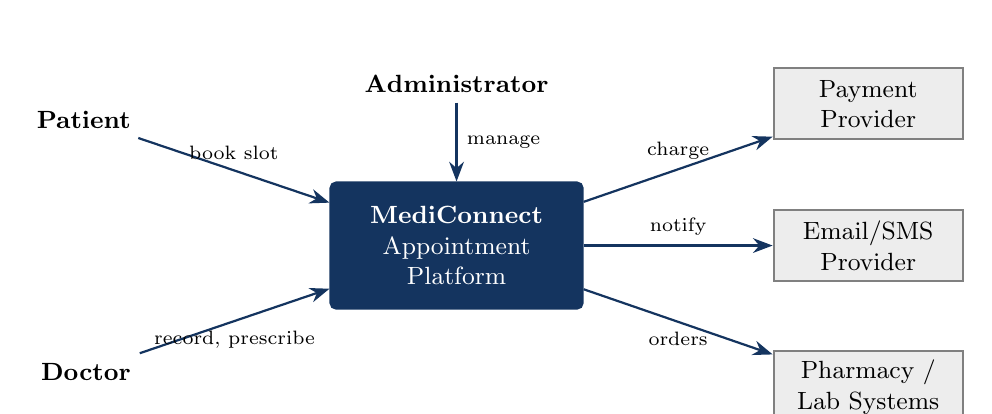
\begin{tikzpicture}[node distance=1.0cm and 2.4cm]
  \node[box,fill=navy,text=white,minimum width=3.2cm,minimum height=1.6cm] (sys) {\textbf{MediConnect}\\Appointment\\Platform};
  \node[actor,left=of sys,yshift=1.6cm] (pat) {\textbf{Patient}};
  \node[actor,left=of sys,yshift=-1.6cm] (doc) {\textbf{Doctor}};
  \node[actor,above=of sys] (admin) {\textbf{Administrator}};
  \node[ext,right=of sys,yshift=1.8cm] (pay) {Payment\\Provider};
  \node[ext,right=of sys] (sms) {Email/SMS\\Provider};
  \node[ext,right=of sys,yshift=-1.8cm] (pharm) {Pharmacy /\\Lab Systems};

  \draw[flow] (pat) -- node[above,font=\scriptsize]{book slot} (sys);
  \draw[flow] (doc) -- node[below,font=\scriptsize]{record, prescribe} (sys);
  \draw[flow] (admin) -- node[right,font=\scriptsize]{manage} (sys);
  \draw[flow] (sys) -- node[above,font=\scriptsize]{charge} (pay);
  \draw[flow] (sys) -- node[above,font=\scriptsize]{notify} (sms);
  \draw[flow] (sys) -- node[below,font=\scriptsize]{orders} (pharm);
\end{tikzpicture}
\caption{Context diagram: MediConnect and its external entities.}
\end{figure}

\subsection{Architecture Diagram}
The high-level architecture organises the system into client, gateway, service, messaging,
and data tiers.

\begin{figure}[H]
\centering
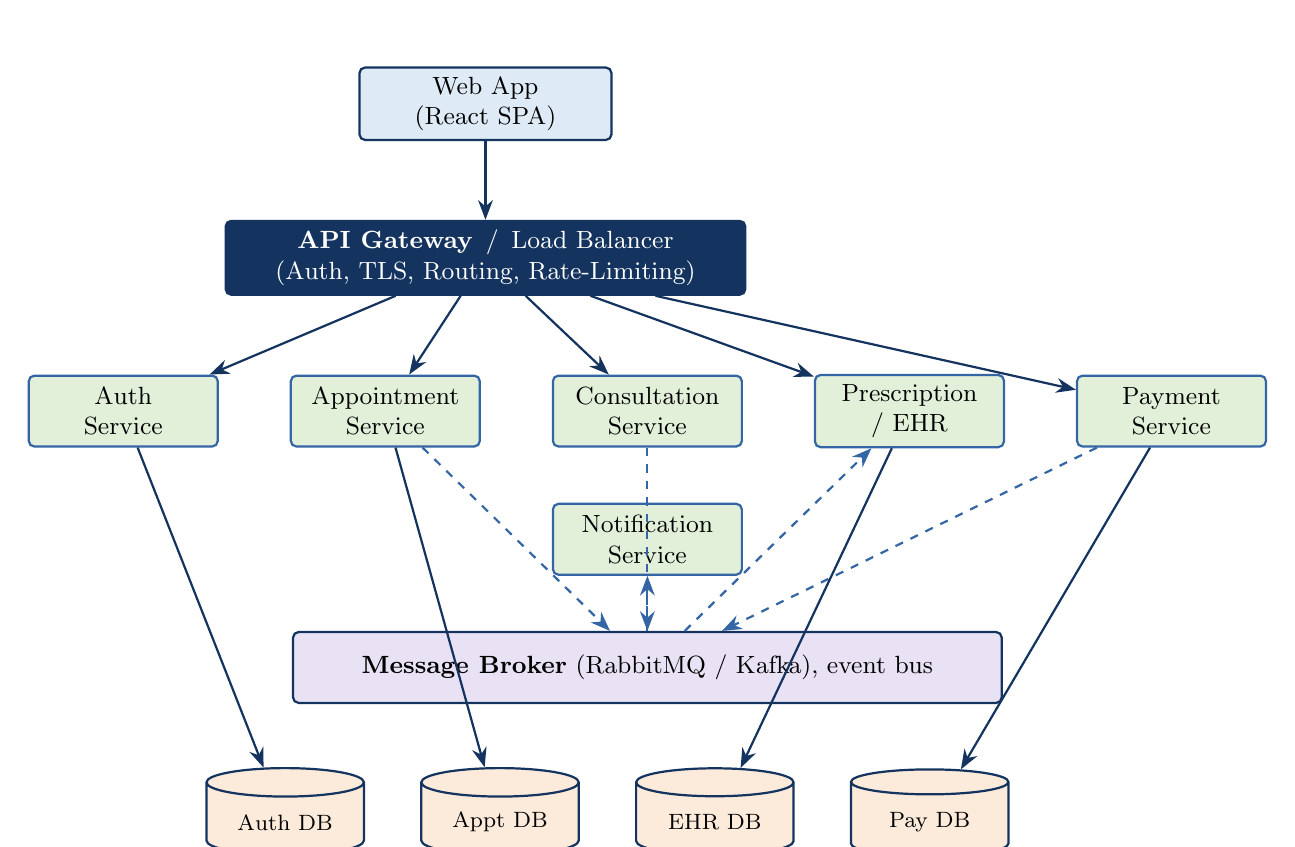
\begin{tikzpicture}[node distance=0.7cm and 0.9cm]
  \node[box,minimum width=3.2cm] (web) {Web App\\(React SPA)};
  \node[box,fill=navy,text=white,minimum width=6.6cm,below=1.0cm of web] (gw) {\textbf{API Gateway} \,/\, Load Balancer\\ (Auth, TLS, Routing, Rate-Limiting)};
  \node[svc,below=1.0cm of gw,xshift=-4.6cm] (auth) {Auth\\Service};
  \node[svc,right=of auth] (appt) {Appointment\\Service};
  \node[svc,right=of appt] (cons) {Consultation\\Service};
  \node[svc,right=of cons] (presc) {Prescription\\/ EHR};
  \node[svc,right=of presc] (payv) {Payment\\Service};
  \node[svc,below=0.7cm of cons] (notif) {Notification\\Service};
  \node[box,fill=softpurple,below=0.7cm of notif,minimum width=9cm] (broker) {\textbf{Message Broker} (RabbitMQ / Kafka), event bus};
  \node[store,below=0.8cm of broker,xshift=-4.6cm] (db1) {Auth DB};
  \node[store,right=0.7cm of db1] (db2) {Appt DB};
  \node[store,right=0.7cm of db2] (db3) {EHR DB};
  \node[store,right=0.7cm of db3] (db4) {Pay DB};

  \draw[flow] (web) -- (gw);
  \draw[flow] (gw) -- (auth);
  \draw[flow] (gw) -- (appt);
  \draw[flow] (gw) -- (cons);
  \draw[flow] (gw) -- (presc);
  \draw[flow] (gw) -- (payv);
  \draw[flowg] (appt) -- (broker);
  \draw[flowg] (cons) -- (broker);
  \draw[flowg] (payv) -- (broker);
  \draw[flowg] (broker) -- (notif);
  \draw[flowg] (broker) -- (presc);
  \draw[flow] (auth) -- (db1);
  \draw[flow] (appt) -- (db2);
  \draw[flow] (presc) -- (db3);
  \draw[flow] (payv) -- (db4);
\end{tikzpicture}
\caption{High-level microservices architecture (solid = synchronous REST, dashed = asynchronous events).}
\end{figure}

\subsection{Component Diagram}
Internally, each service follows a layered structure (controller, business logic, data
access), so that upper layers do not bypass lower ones. For example, the controller never
accesses the database directly. The figure details the \textbf{Appointment Service} as a
representative example.

\begin{figure}[H]
\centering
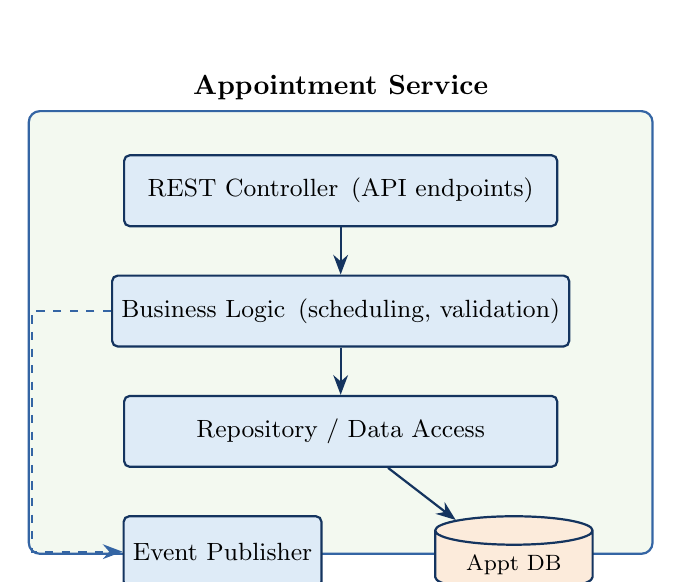
\begin{tikzpicture}[node distance=0.8cm]
  \begin{scope}[on background layer]
    \node[draw=steel,thick,rounded corners,fill=softgreen!40,fit={(0,0) (7.5,5.2)},inner sep=6pt,label=above:{\textbf{Appointment Service}}] {};
  \end{scope}
  \node[box,minimum width=5.5cm] (ctrl) at (3.75,4.4) {REST Controller \,(API endpoints)};
  \node[box,minimum width=5.5cm,below=0.6cm of ctrl] (logic) {Business Logic \,(scheduling, validation)};
  \node[box,minimum width=5.5cm,below=0.6cm of logic] (repo) {Repository / Data Access};
  \node[box,minimum width=2.5cm,below=0.6cm of repo,xshift=-1.5cm] (evt) {Event Publisher};
  \node[store,below=0.6cm of repo,xshift=2.2cm,minimum height=0.9cm] (db) {Appt DB};
  \draw[flow] (ctrl) -- (logic);
  \draw[flow] (logic) -- (repo);
  \draw[flow] (repo) -- (db);
  \draw[flowg] (logic.west) -- ++(-1.0,0) |- (evt.west);
\end{tikzpicture}
\caption{Component decomposition of a representative microservice (Appointment Service).}
\end{figure}

\subsection{Deployment Diagram}
Services are containerised and orchestrated on a Kubernetes cluster, with managed databases
and a CDN for the web client.

\begin{figure}[H]
\centering
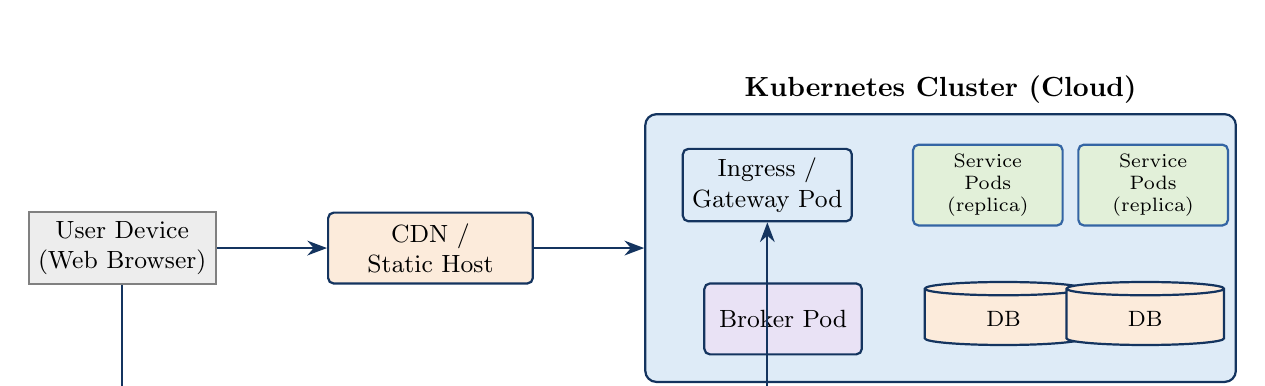
\begin{tikzpicture}[node distance=0.7cm and 1.0cm]
  \node[ext,minimum width=2.2cm] (client) {User Device\\(Web Browser)};
  \node[box,fill=softorange,right=1.4cm of client] (cdn) {CDN /\\Static Host};
  \node[draw=navy,thick,rounded corners,fill=lightblue,minimum width=7.5cm,minimum height=3.4cm,right=1.4cm of cdn,label=above:{\textbf{Kubernetes Cluster (Cloud)}}] (k8s) {};
  \node[box,minimum width=2.0cm] at ([yshift=0.8cm,xshift=-2.2cm]k8s.center) (n1) {Ingress /\\Gateway Pod};
  \node[svc,minimum width=1.9cm,font=\scriptsize] at ([yshift=0.8cm,xshift=0.6cm]k8s.center) (n2) {Service\\Pods\\(replica)};
  \node[svc,minimum width=1.9cm,font=\scriptsize] at ([yshift=0.8cm,xshift=2.7cm]k8s.center) (n3) {Service\\Pods\\(replica)};
  \node[box,fill=softpurple,minimum width=2.0cm] at ([yshift=-0.9cm,xshift=-2.0cm]k8s.center) (mb) {Broker Pod};
  \node[store,minimum height=0.8cm] at ([yshift=-0.9cm,xshift=0.8cm]k8s.center) (dba) {DB};
  \node[store,minimum height=0.8cm] at ([yshift=-0.9cm,xshift=2.6cm]k8s.center) (dbb) {DB};

  \draw[flow] (client) -- (cdn);
  \draw[flow] (cdn) -- (k8s.west|-cdn);
  \draw[flow] (client.south) |- ([yshift=-1.4cm]client.south) -| (n1.south);
\end{tikzpicture}
\caption{Deployment view: containerised services on a managed Kubernetes cluster.}
\end{figure}

\subsection{Class Diagram}
The core domain entities and their relationships are shown below (attributes abbreviated). An
appointment is booked by a patient, is with a doctor, and takes place at a clinic.

\begin{figure}[H]
\centering
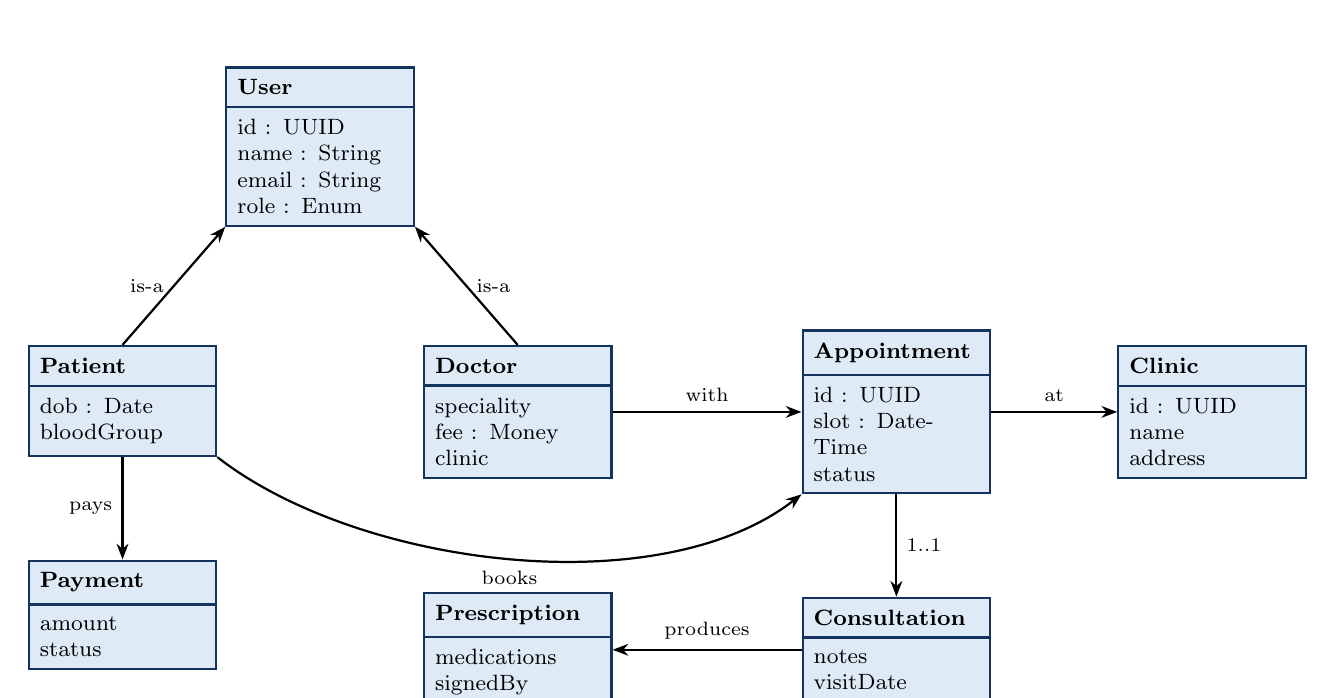
\begin{tikzpicture}[
   class/.style={rectangle split,rectangle split parts=2,draw=navy,thick,
                 fill=lightblue,font=\footnotesize,inner sep=4pt,text width=2.1cm,align=left},
   rel/.style={-{Stealth[length=2mm]},thick}
]
  \node[class] (user)
     {\textbf{User}\nodepart{second}id : UUID\\ name : String\\ email : String\\ role : Enum};
  \node[class,below left=1.5cm and 0.1cm of user] (patient)
     {\textbf{Patient}\nodepart{second}dob : Date\\ bloodGroup};
  \node[class,below right=1.5cm and 0.1cm of user] (doctor)
     {\textbf{Doctor}\nodepart{second}speciality\\ fee : Money\\ clinic};
  \node[class,right=2.4cm of doctor] (appt)
     {\textbf{Appointment}\nodepart{second}id : UUID\\ slot : DateTime\\ status};
  \node[class,right=1.6cm of appt] (clinic)
     {\textbf{Clinic}\nodepart{second}id : UUID\\ name\\ address};
  \node[class,below=1.3cm of appt] (consult)
     {\textbf{Consultation}\nodepart{second}notes\\ visitDate};
  \node[class,left=2.4cm of consult] (presc)
     {\textbf{Prescription}\nodepart{second}medications\\ signedBy};
  \node[class,below=1.3cm of patient] (pay)
     {\textbf{Payment}\nodepart{second}amount\\ status};

  \draw[rel] (patient.north) -- (user.south west) node[midway,left,font=\scriptsize]{is-a};
  \draw[rel] (doctor.north) -- (user.south east) node[midway,right,font=\scriptsize]{is-a};
  \draw[rel] (patient.south east) .. controls +(1.8,-1.4) and +(-1.8,-1.4) .. (appt.south west)
        node[pos=0.5,below=1pt,font=\scriptsize]{books};
  \draw[rel] (doctor.east) -- (appt.west) node[midway,above,font=\scriptsize]{with};
  \draw[rel] (appt.east) -- (clinic.west) node[midway,above,font=\scriptsize]{at};
  \draw[rel] (appt.south) -- (consult.north) node[midway,right,font=\scriptsize]{1..1};
  \draw[rel] (consult.west) -- (presc.east) node[midway,above,font=\scriptsize]{produces};
  \draw[rel] (patient.south) -- (pay.north) node[midway,left,font=\scriptsize]{pays};
\end{tikzpicture}
\caption{Domain class diagram (core entities and relationships).}
\end{figure}

\subsection{Data Flow Diagram}
The following data flow diagram (Level~1) traces the ``search, book, and pay for an
appointment'' flow and shows how the components interact at run time.

\begin{figure}[H]
\centering
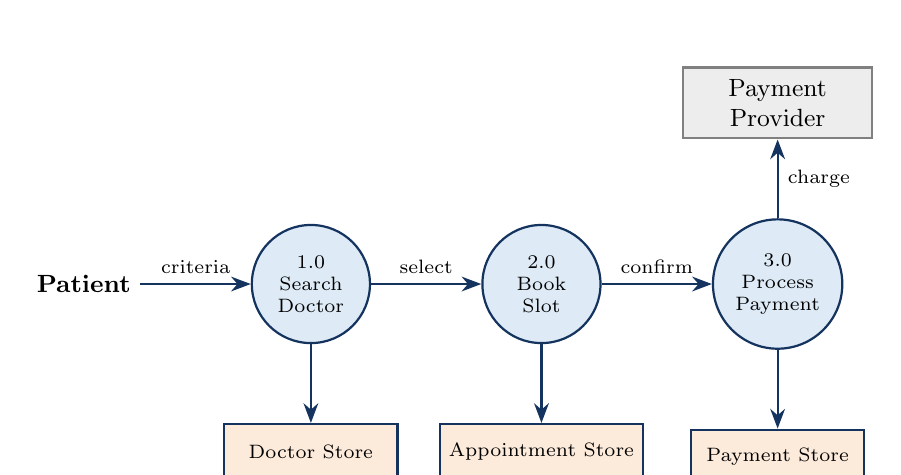
\begin{tikzpicture}[node distance=1.0cm and 1.4cm,
   proc/.style={circle,draw=navy,thick,fill=lightblue,minimum size=1.5cm,align=center,font=\scriptsize},
   ds/.style={draw=navy,thick,fill=softorange,minimum width=2.2cm,minimum height=0.7cm,align=center,font=\scriptsize}]
  \node[actor] (pat) {\textbf{Patient}};
  \node[proc,right=of pat] (p1) {1.0\\Search\\Doctor};
  \node[proc,right=of p1] (p2) {2.0\\Book\\Slot};
  \node[proc,right=of p2] (p3) {3.0\\Process\\Payment};
  \node[ds,below=of p1] (d1) {Doctor Store};
  \node[ds,below=of p2] (d2) {Appointment Store};
  \node[ds,below=of p3] (d3) {Payment Store};
  \node[ext,above=of p3] (gw) {Payment\\Provider};

  \draw[flow] (pat) -- node[above,font=\scriptsize]{criteria} (p1);
  \draw[flow] (p1) -- (d1);
  \draw[flow] (p1) -- node[above,font=\scriptsize]{select} (p2);
  \draw[flow] (p2) -- (d2);
  \draw[flow] (p2) -- node[above,font=\scriptsize]{confirm} (p3);
  \draw[flow] (p3) -- (d3);
  \draw[flow] (p3) -- node[right,font=\scriptsize]{charge} (gw);
\end{tikzpicture}
\caption{Level-1 data flow diagram for the search, booking, and payment process.}
\end{figure}

% ============================================================
\section{Technology Stack Selection}
The stack is chosen to support the microservices style, polyglot persistence, and consistent
operational tooling.

\begin{longtable}{p{3.6cm} p{4.6cm} p{5.4cm}}
\caption{Technology stack and rationale.}\\
\toprule
\textbf{Layer} & \textbf{Technology} & \textbf{Rationale}\\
\midrule
\endfirsthead
\toprule
\textbf{Layer} & \textbf{Technology} & \textbf{Rationale}\\
\midrule
\endhead
Front-end & React.js + TypeScript & Component-based, responsive single-page web app.\\
API Gateway & Kong / NGINX & Central auth, routing, TLS termination, rate limiting.\\
Backend services & Node.js (Express) and Spring Boot & Lightweight services in Node; Spring
Boot where strong typing and transactions matter.\\
Messaging & RabbitMQ / Apache Kafka & Asynchronous, decoupled event delivery.\\
Databases & PostgreSQL (transactional), MongoDB (records) & Polyglot persistence,
database-per-service.\\
Caching & Redis & Session and token cache, doctor and slot availability cache.\\
Authentication & JWT + OAuth 2.0 & Stateless, role-based access tokens.\\
Containerisation & Docker + Kubernetes & Packaging, orchestration, auto-scaling, self-healing.\\
CI/CD & GitHub Actions / Jenkins & Automated build, test, and deploy pipelines.\\
Monitoring & Prometheus + Grafana, ELK & Metrics, dashboards, centralised logging.\\
Cloud & AWS / Azure & Managed Kubernetes, databases, and CDN.\\
\bottomrule
\end{longtable}

% ============================================================
\section{Quality Attributes}
This section explains how the design addresses each required quality attribute.

\subsection{Scalability}
Each microservice is stateless behind the gateway and deployed as multiple replicas.
Kubernetes' Horizontal Pod Autoscaler adds or removes pods based on CPU and latency, so the
appointment booking service can scale on its own during peak times, separately from lighter
services. Redis caching and the database-per-service pattern remove shared bottlenecks,
satisfying NFR-01.

\subsection{Performance}
The API Gateway routes efficiently and offloads TLS, and Redis caches frequent reads such as
doctor listings and slot availability, which keeps the median request below the 500\,ms target.
Database indexing on doctor, clinic, and slot fields keeps search and booking queries fast
(NFR-02).

\subsection{Security}
Security is applied in layers (defence in depth): TLS 1.2+ for all traffic, JWT and OAuth\,2.0
with role-based access control at the gateway, encryption at rest for records and payment data,
input validation in each service, and audit logging. The payment service is isolated and never
stores raw card data, delegating to a secure payment provider (NFR-03, NFR-07).

\subsection{Availability}
Replicated, stateless services and Kubernetes self-healing remove single points of failure.
The message broker decouples services, so a temporary outage of the notification service does
not block bookings; events are queued and processed when it recovers. Multi-zone deployment
supports the 99.9\% uptime goal (NFR-04).

\subsection{Maintainability}
Clear service boundaries, well-defined interfaces, and independent CI/CD pipelines let teams
change and deploy one service without redeploying the whole system. Containerisation gives
consistent environments from development to production (NFR-06).

\subsection{Reliability}
Critical operations such as booking, payment, and prescription use transactional databases and
the Saga pattern for consistency across services, with compensating actions on failure. Retries
with idempotency keys and durable message queues ensure that events are not lost, and health
checks restart failed services automatically (NFR-05).

\begin{longtable}{p{3.2cm} p{4.4cm} p{6.0cm}}
\caption{Mapping of quality attributes to architectural tactics.}\\
\toprule
\textbf{Quality Attribute} & \textbf{Architectural Tactic} & \textbf{Realised By}\\
\midrule
\endfirsthead
\toprule
\textbf{Quality Attribute} & \textbf{Architectural Tactic} & \textbf{Realised By}\\
\midrule
\endhead
Scalability & Horizontal replication & K8s HPA, stateless services, Redis\\
Performance & Caching, edge routing & Redis, API Gateway, database indexing\\
Security & Defence in depth & TLS, JWT/OAuth, RBAC, encryption, audit logs\\
Availability & Redundancy and isolation & Replicas, self-healing, message broker\\
Maintainability & Modularity & Microservices, clear interfaces, CI/CD\\
Reliability & Consistency and recovery & Saga pattern, idempotency, health checks\\
\bottomrule
\end{longtable}

% ============================================================
\section{Conclusion}
This report analysed the problem of manual, queue-based appointment handling at clinics and
proposed \textbf{MediConnect}, a web platform that lets patients book appointments with clinic
doctors in advance and then attend in person. The system is built on a microservices
architecture with an API Gateway, an event-driven message bus, and a layered organisation inside
each service. The requirements analysis identified the functional and non-functional
requirements and the stakeholders they serve, and a comparison of common architecture styles
showed that microservices best satisfy this system's needs for independent scalability, fault
isolation, security, and maintainability.

The design was presented through context, architecture, component, deployment, class, and
data-flow diagrams, and supported by a practical technology stack. The main architectural
decisions, namely the use of microservices, a central API Gateway, a database-per-service model,
and an event-driven backbone, were justified against the system goals, and each quality attribute
was traced to a concrete design tactic. The scope was kept focused so that the core
functionalities can be built as a working prototype. The result is an architecture that is
scalable, secure, available, and maintainable, and that provides a clear foundation for
implementation.

\end{document}
